%Este trabalho está licenciado sob a Licença Atribuição-CompartilhaIgual 4.0 Internacional Creative Commons. Para visualizar uma cópia desta licença, visite http://creativecommons.org/licenses/by-sa/4.0/deed.pt_BR ou mande uma carta para Creative Commons, PO Box 1866, Mountain View, CA 94042, USA.

\chapter{Bases e coordenadas}\label{cap_base}
\thispagestyle{fancy}

\section{Dependência linear}\label{cap_base_sec_deplinear}

\subsection{Combinação linear}

Dados vetores $\vec{u}_1$, $\vec{u}_2$, $\dotsc$, $\vec{u}_n$ e números reais $c_1$, $c_2$, $\dotsc$, $c_n$, com $n$ inteiro positivo, chamamos de
\begin{equation}
  \vec{u} = c_1\vec{u}_1 + c_2\vec{u}_2 + \cdots + c_n\vec{u}_n
\end{equation}
uma {\bf combinação linear}\index{combinação linear} de $\vec{u}_1$, $\vec{u}_2$, $\dotsc$, $\vec{u}_n$. Neste caso, também dizemos que $\vec{u}$ é {\bf gerado} pelos vetores $\vec{u}_1$, $\vec{u}_2$, $\dotsc$, $\vec{u}_n$ ou, equivalentemente, que estes vetores {\bf geram} o vetor $\vec{u}$.

\begin{ex}\label{ex:comblinear}
  Sejam dados os vetores $\vec{v}$, $\vec{w}$ e $\vec{z}$. Então, temos:
  \begin{itemize}
  \item $\vec{u}_1 = \frac{1}{2}\vec{u} + \sqrt{2}\vec{z}$ é uma combinação linear dos vetores $\vec{v}$ e $\vec{z}$.
  \item $\vec{u_2} = \vec{u} - 2\vec{z}$ é uma outra combinação linear dos vetores $\vec{v}$ e $\vec{z}$.
  \item $\vec{u_3} = 2\vec{u} - \vec{w} + \pi\vec{z}$ é uma combinação linear dos vetores $\vec{u}$, $\vec{w}$ e $\vec{z}$.
  \item $\vec{u_4} = \frac{3}{2}\vec{z}$ é uma combinação linear do vetor $\vec{z}$.
  \end{itemize}
\end{ex}

\subsection{Dependência linear}

Dois ou mais vetores dados são {\bf linearmente dependentes}\index{linearmente!dependente} (abreviação, l.d.) quando um deles for combinação linear dos demais.

\begin{ex}\label{ex:deplinear}
  No exemplo anterior (Exemplo \ref{ex:comlinear}), temos:
  \begin{itemize}
  \item $\vec{u_1}$ e $\vec{u_2}$ dependem linearmente dos vetores $\vec{u}$ e $\vec{z}$.
  \item $\vec{u_3}$ depende linearmente dos vetores $\vec{u}$, $\vec{v}$ e $\vec{z}$.
  \item Os vetores $\vec{u_4}$ e $\vec{z}$ são linearmente dependentes.
  \end{itemize}
\end{ex}

Dois ou mais vetores dados são {\bf linearmente independentes}\index{linearmente!independentes} (abreviação, l.i.)quando eles não são linearmente dependentes.

\subsection{Observações}

\subsubsection{Dois vetores}

Dois vetores quaisquer $\vec{u}\neq\vec{0}$ e $\vec{v}\neq\vec{0}$ são l.d. se, e somente se, qualquer uma das seguinte condições é satisfeita:
\begin{itemize}
\item um deles é combinação linear do outro, i.e.
  \begin{equation}
    \vec{u} = \alpha\vec{v}\quad\text{ou}\quad\vec{v}=\beta\vec{u};
  \end{equation}
\item $\vec{u}$ e $\vec{v}$ têm a mesma direção;
\item $\vec{u}$ e $\vec{v}$ são paralelos.
\end{itemize}

\begin{obs}
  O vetor nulo $\vec{0}$ é l.d. a qualquer vetor $\vec{u}$. De fato, temos
  \begin{equation}
    \vec{0} = 0\cdot\vec{u},
  \end{equation}
  i.e. o vetor nulo é combinação linear do vetor $\vec{u}$.
\end{obs}

\begin{obs}
  Dois vetores não nulos $\vec{u}$ e $\vec{v}$ são l.i. se, e somente se,
  \begin{equation}
    \alpha\vec{u} + \beta\vec{v} = 0 \Rightarrow \alpha=\beta=0.
  \end{equation}
  De fato, se $\alpha\neq 0$, então podemos escrever
  \begin{equation}
    \vec{u} = -\frac{\beta}{\alpha}\vec{v},
  \end{equation}
  i.e. o vetor $\vec{u}$ é combinação linear do vetor $\vec{v}$ e, portanto, estes vetores são l.d.. Isto contradiz a hipótese de eles serem l.i.. Analogamente, se $\beta \neq 0$, então podemos escrever
  \begin{equation}
    \vec{v} = -\frac{\alpha}{\beta}\vec{u}
  \end{equation}
  e, então, teríamos $\vec{u}$ e $\vec{v}$ l.d..
\end{obs}


\subsubsection{Três vetores}

Três vetores quaisquer $\vec{u}$, $\vec{v}$ e $\vec{w}$ são l.d. quando um deles pode ser escrito como combinação linear dois outros dois. Sem perda de generalidade, isto significa que existem constantes $\alpha$ e $\beta$ tais que
\begin{equation}
  \vec{u} = \alpha\vec{v} + \beta\vec{w}.
\end{equation}

Afirmamos que se $\vec{u}$, $\vec{v}$ e $\vec{w}$ são l.d., então $\vec{u}$, $\vec{v}$ e $\vec{w}$ são coplanares. Do fato de que dois vetores quaisquer são sempre coplanares, temos que $\vec{u}$, $\vec{v}$ e $\vec{w}$ são coplanares caso qualquer um deles seja o vetor nulo. Suponhamos, agora, que $\vec{u}$, $\vec{v}$ e $\vec{w}$ são não nulos e seja $\pi$ o plano determinado pelos vetores $\vec{v}$ e $\vec{w}$. Se $\alpha = 0$, então $\vec{u} = \beta\vec{w}$ e teríamos uma representação de $\vec{u}$ no plano $\pi$. Analogamente, se $\beta=0$, então $\vec{u} = \alpha\vec{v}$ e teríamos uma representação de $\vec{u}$ no plano $\pi$. Por fim, observemos que se $\alpha,\beta\neq 0$, então $\alpha\vec{v}$ tem a mesma direção de $\vec{v}$ e $\beta\vec{w}$ tem a mesma direção de $\vec{w}$. Isto é, $\alpha\vec{v}$ e $\beta\vec{w}$ admitem representações no plano $\pi$. Sejam $\overrightarrow{AB}$ e $\overrightarrow{BC}$ representações dos vetores $\alpha\vec{v}$ e $\beta\vec{w}$, respectivamente. Os pontos $A$, $B$ e $C$ pertencem a $\pi$, assim como o segmento $AC$. Como $\overrightarrow{AC} = \vec{u} = \alpha\vec{v} + \beta\vec{w}$, concluímos que $\vec{u}$, $\vec{v}$ e $\vec{w}$ são coplanares.

Reciprocamente, se $\vec{u}$, $\vec{v}$ e $\vec{w}$ são coplanares, então $\vec{u}$, $\vec{v}$ e $\vec{w}$ são l.d.. De fato, se um deles for nulo, por exemplo, $\vec{u}=\vec{0}$, então $\vec{u}$ pode ser escrito como a seguinte combinação linear dos vetores $\vec{v}$ e $\vec{w}$
\begin{equation}
  \vec{u} = 0\vec{v} + 0\vec{w}.
\end{equation}
Neste caso, $\vec{u}$, $\vec{v}$ e $\vec{w}$ são l.d.. Também, se dois dos vetores forem paralelos, por exemplo, $\vec{u}\parallel\vec{v}$, então temos a combinação linear
\begin{equation}
  \vec{u} = \alpha\vec{v} + 0\vec{w}.
\end{equation}
E, então, $\vec{u}$, $\vec{v}$ e $\vec{w}$ são l.d.. Agora, suponhamos que $\vec{u}$, $\vec{v}$ e $\vec{w}$ são não nulos e dois a dois concorrentes. Sejam, então $\overrightarrow{PA}=\vec{u}$, $\overrightarrow{PB}=\vec{v}$ e $\overrightarrow{PC}=\vec{w}$ representações sobre um plano $\pi$. Sejam $r$ e $s$ as retas determinadas por $PA$ e $PC$, respectivamente. Seja, então, $D$ o ponto de interseção da reta $s$ com a reta paralela a $r$ que passa pelo ponto $B$. Seja, também, $E$ o ponto de interseção da reta $r$ com a reta paralela a $s$ que passa pelo ponto $B$. Sejam, então, $\alpha$ e $\beta$ tais que $\alpha\vec{u}=\overrightarrow{PE}$ e $\beta\vec{w}=\overrightarrow{PD}$. Como $\vec{v} = \overrightarrow{PB} = \overrightarrow{PE} + \overrightarrow{PD} = \alpha\vec{u}+\beta\vec{w}$, temos que $\vec{v}$ é combinação linear de $\vec{u}$ e $\vec{w}$, i.e. $\vec{u}$, $\vec{v}$ e $\vec{w}$ são l.d..

\begin{obs}
  Três vetores dados $\vec{u}$, $\vec{v}$ e $\vec{w}$ são l.i. se, e somente se, 
  \begin{equation}
    \alpha\vec{u} + \beta\vec{v} + \gamma\vec{w} = 0 \Rightarrow \alpha=\beta=\gamma = 0.
  \end{equation}
  De fator, sem perda de generalidade, se $\alpha\neq 0$, podemos escrever
  \begin{equation}
    \vec{u} = -\frac{\beta}{\alpha}\vec{v} - \frac{\gamma}{\alpha}\vec{w},
  \end{equation}
  e teríamos $\vec{u}$, $\vec{v}$ e $\vec{w}$ vetores l.d..
\end{obs}

\subsubsection{Quatro ou mais vetores}

{\bf Quatro ou mais vetores são sempre l.d..} De fato, sejam dados quatro vetores $\vec{a}$, $\vec{b}$, $\vec{c}$ e $\vec{d}$. Se dois ou três destes forem l.d. entre si, então, por definição, os quatro são l.d.. Assim sendo, suponhamos que três dos vetores sejam l.i. e provaremos que, então, o outro vetor é combinação linear desses três.

Sem perda de generalidade, suponhamos que $\vec{a}$, $\vec{b}$ e $\vec{c}$ são l.i.. Logo, eles não são coplanares. Seja, ainda, $\pi$ o plano determinado pelos vetores $\vec{a}$, $\vec{b}$ e as representações $\vec{a}=\overrightarrow{PA}$, $\vec{b}=\overrightarrow{PB}$, $\vec{c}=\overrightarrow{PC}$ e $\vec{d}=\overrightarrow{PD}$.

\begin{figure}[H]
  \centering
  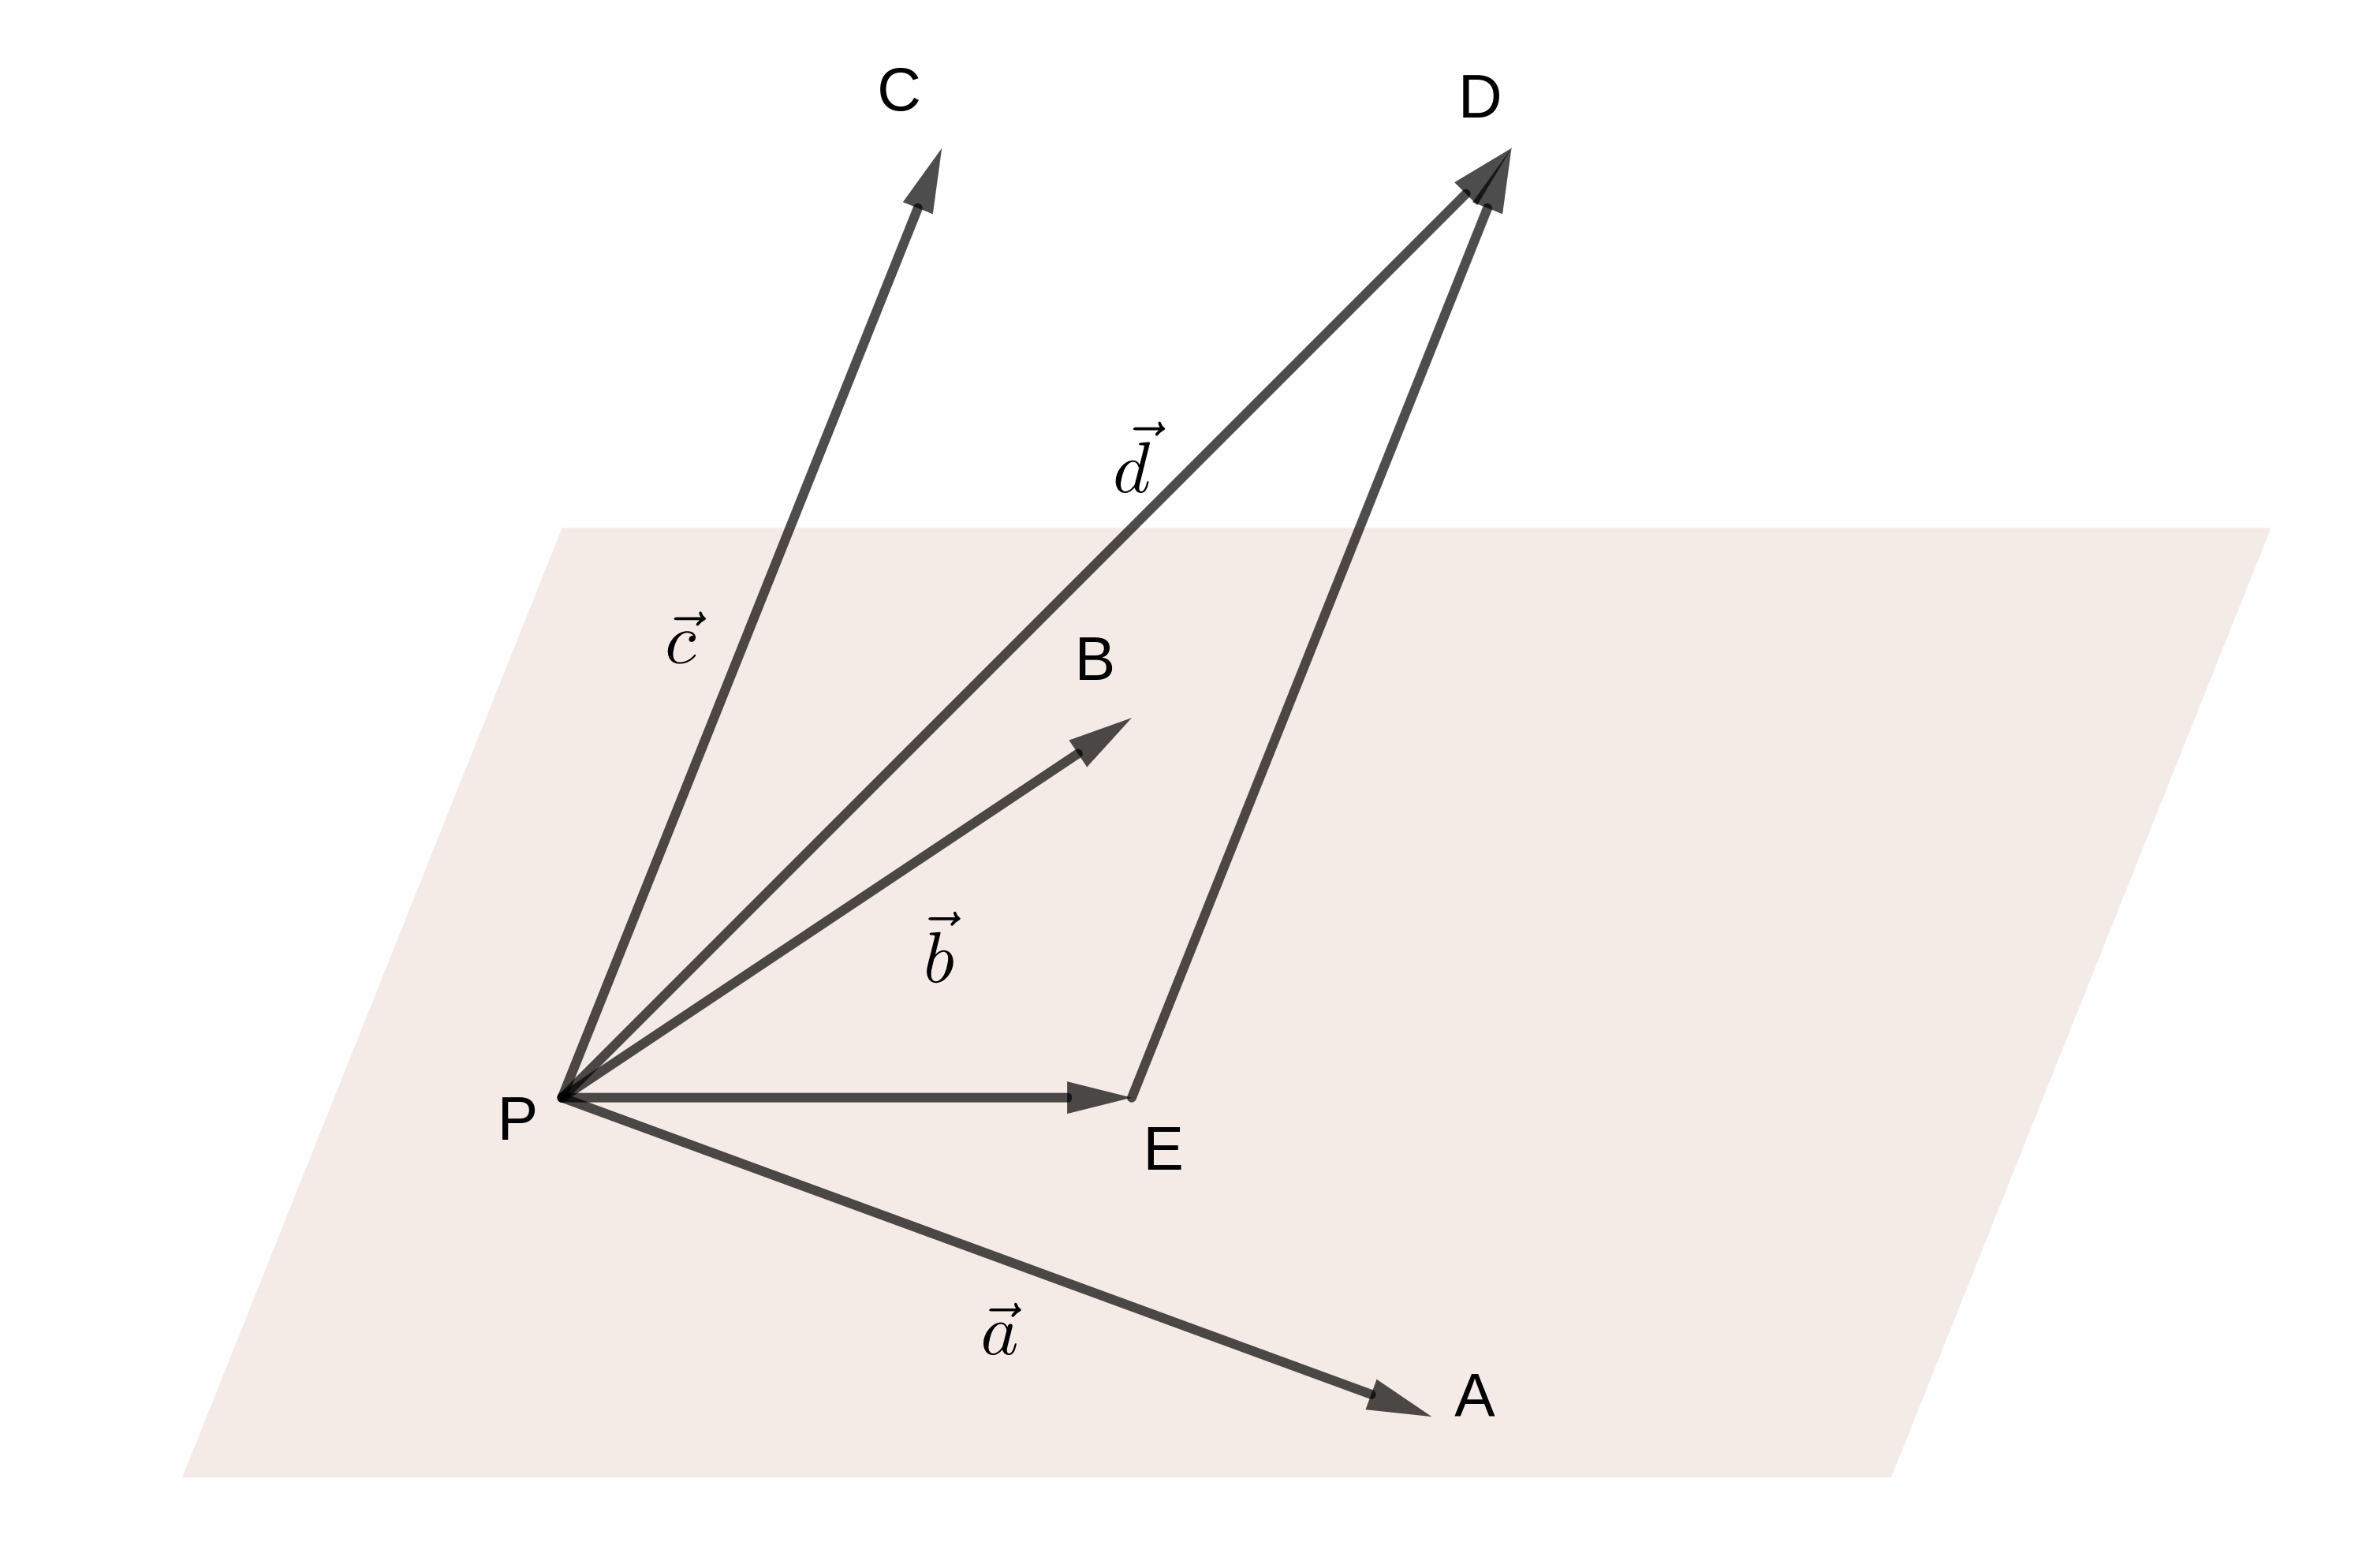
\includegraphics[width=0.7\textwidth]{./cap_base/dados/fig_4vec_ld/fig_4vec_ld}
  \caption{Quatro vetores são l.d..}
  \label{fig:4vec_ld}
\end{figure}

Consideremos a reta $r$ paralela a $\overrightarrow{PC}$ que passa pelo ponto $D$. Então, seja $E$ o ponto de interseção de $r$ com o plano $\pi$. Vejamos a Figura \ref{fig:}. Observamos que o vetor $\overrightarrow{PE}$ é coplanar aos vetores $\overrightarrow{PA}$ e $\overrightarrow{PB}$ e, portanto, exitem números reais $alpha$ e $\beta$ tal que
\begin{equation}
  \overrightarrow{PE} = \alpha\overrightarrow{PA} + \beta\overrightarrow{PB}.
\end{equation}
Além disso, como $\overrightarrow{ED}$ tem a mesma direção e sentido de $\overrightarrow{PC} = \vec{c}$, temos que
\begin{equation}
  \overrightarrow{ED} = \gamma\overrightarrow{PC}
\end{equation}
para algum número real $\gamma$. Por fim, observamos que
\begin{align*}
  \overrightarrow{PD} &= \overrightarrow{PE} + \overrightarrow{ED}\\
                      &= \alpha\overrightarrow{PA} + \beta\overrightarrow{PB} + \gamma\overrightarrow{PC}\\
                      &= \alpha\vec{a} + \beta\vec{b} + \gamma\vec{c}.
\end{align*}

\subsection*{Exercícios}

\emconstrucao
